\documentclass{beamer}
\usepackage[utf8]{inputenc}
\usepackage{graphicx}
\usepackage{hyperref}
\usepackage{relsize}

\title{Documentação de Código em Python}
\author{Eduardo Ribeiro Silva de Oliveira}
\date{07 de Outubro de 2024}

\begin{document}

\frame{\titlepage}

\begin{frame}
  \frametitle{O que é documentação de código?}
  \begin{itemize}
    \item Registrar funcionalidades, finalidades, entradas, saídas e dependências.
    \item Ajudar na manutenção e compreensão do código.
  \end{itemize}
\end{frame}

\begin{frame}
  \frametitle{Por que é importante?}
  \begin{itemize}
    \item Facilita manutenção e colaboração.
    \item Reduz erros ao melhorar a compreensão do fluxo de dados.
  \end{itemize}
\end{frame}

\begin{frame}
  \frametitle{Como otimizar a documentação?}
  \begin{itemize}
    \item Escrever códigos intuitivos.
    \item Seguir um padrão.
    \item Utilizar ferramentas automatizadas.
  \end{itemize}
\end{frame}

\begin{frame}
  \frametitle{Auto-documentação por Valdemar W. Setzer}
  \begin{itemize}
    \item Proposta para adicionar informações detalhadas diretamente no código.
    \item Facilita a consulta de documentação sem outros documentos.
    \item Mais informações: \url{https://www.ime.usp.br/~vwsetzer/Autodoc-de-programas.pdf}
    \item Nível 1: Informações gerais dos procedimentos.
    \item Nível 2: Documentação de nível 1 e os pseudo-códigos.
    \item Nível 3: Todo o código fonte do programa.
  \end{itemize}
\end{frame}

\begin{frame}[fragile]
  \frametitle{Exemplo de Cabeçalho}
  \tiny
  \begin{verbatim}

#1[
#1 TITULO: NOME DO PROGRAMA OU NOME DO ARQUIVO
#1 AUTOR: AUTOR DO ARQUIVO
#1 DATA: DATA DA VERSÃO ATUAL
#1 VERSAO: NÚMERO DA VERSÃO ATUAL
#1 FINALIDADE: EXPLICAÇÃO DO QUE O PROGRAMA FAZ
#1 ENTRADAS: INDICA AS ENTRADAS NECESSÁRIAS PARA A EXECUÇÃO
#1 SAIDAS: INDICA A SAÍDA DO PROGRAMA
#1 ROTINAS CHAMADAS: INDICA AS ROTINAS USADAS
#1]

  \end{verbatim}
  \normalsize
\end{frame}

\begin{frame}[fragile]
  \frametitle{Exemplo de Documentação de Função}
  \tiny
  \begin{verbatim}

    #1[
    #1 ROTINA: __INIT__
    #1 FINALIDADE: INICIALIZA AS VARIÁVEIS DA CLASSE EXTRACTOR
    #1 ENTRADAS: CAMINHO DO ARQUIVO/DIRETÓRIO DE ENTRADA, CAMINHO DO 
    #1 ARQUIVO DE SAÍDA, MODO DE EXECUÇÃO
    #1 DEPENDENCIAS: OS
    #1 CHAMADO POR: EXTRACTOR
    #1 CHAMA: _GET_ALL_FILES (SE O CAMINHO FOR UM DIRETÓRIO)
    #1]
    #2[
    #2 PSEUDOCODIGO DE: __init__
    def __init__(self, input_path: str, output_path: str, execution_mode: int = 3):
        #2 ARMAZENA O CAMINHO DE ENTRADA E O CAMINHO DE SAÍDA
        self.input_path = input_path
        self.output_path = output_path
        #2 DEFINE O MODO DE EXECUÇÃO PADRÃO COMO 3
        self.execution_mode = execution_mode
        #2 VERIFICA SE O CAMINHO DE ENTRADA É UM ARQUIVO ÚNICO
        self.one_file = os.path.isfile(input_path)
        #2 GERA UMA LISTA DE ARQUIVOS A SEREM PROCESSADOS (SE FOR UM DIRETÓRIO)
        self.file_path_list = [input_path] if self.one_file else self._get_all_files(input_path)
        #2 INICIALIZA UM DICIONÁRIO PARA ARMAZENAR A DOCUMENTAÇÃO
        self.documentation = {}
        #2 INICIALIZA UMA STRING VAZIA PARA O CONTEÚDO HTML
        self.html_content = ''  # Armazenará o HTML gerado
    #2]

  \end{verbatim}
  \normalsize
\end{frame}

\begin{frame}
  \frametitle{Imagens de Exemplos}
  \begin{figure}
    \centering
    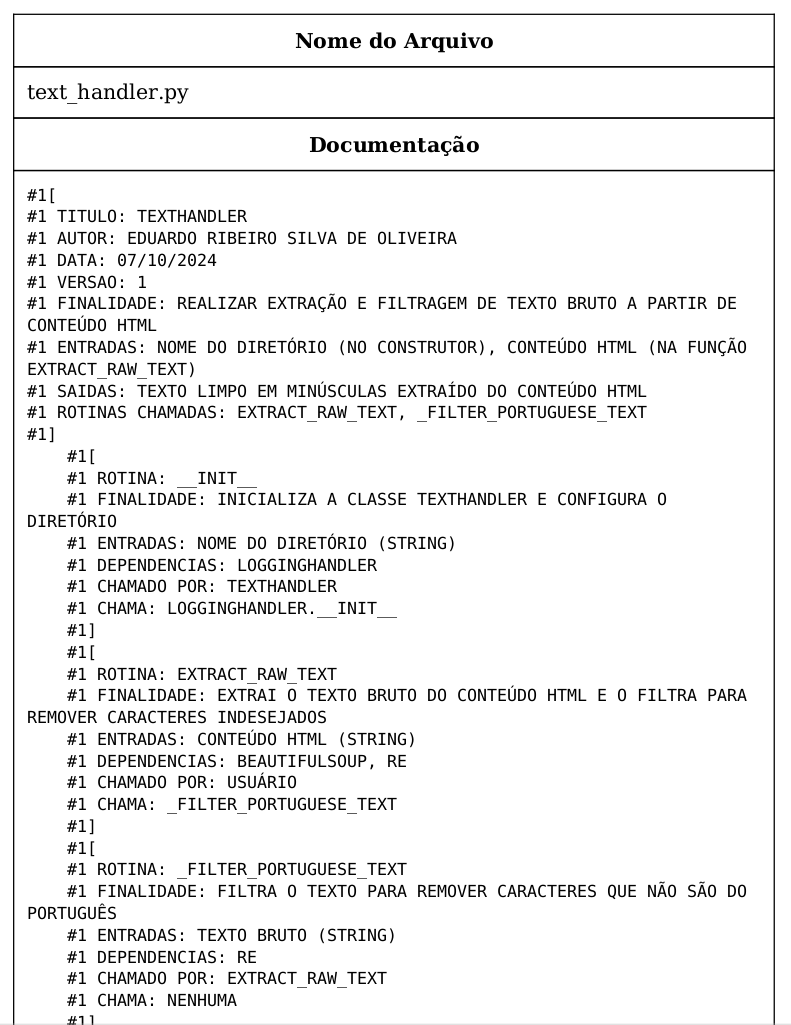
\includegraphics[width=0.7\linewidth]{nivel1.png}
    \caption{Exemplo de visualização de nível 1}
  \end{figure}
\end{frame}

\begin{frame}
  \frametitle{Imagens de Exemplos - Nível 2}
  \begin{figure}
    \centering
    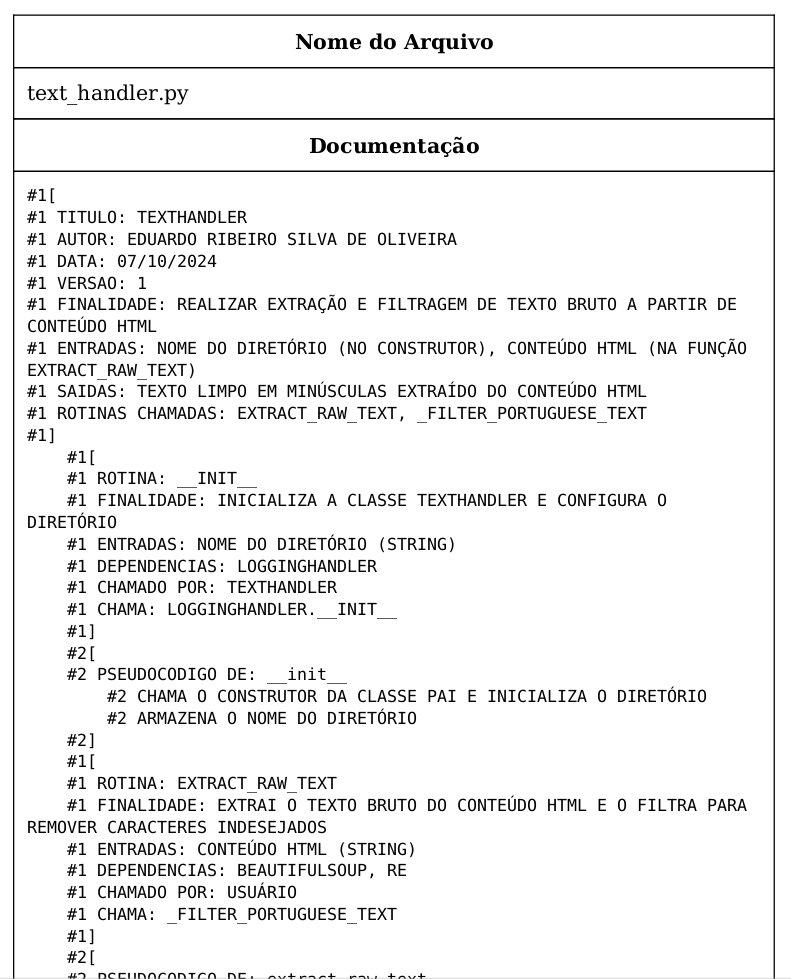
\includegraphics[width=0.7\linewidth]{nivel2.png}
    \caption{Exemplo de visualização de nível 2}
  \end{figure}
\end{frame}

\begin{frame}
  \frametitle{Imagens de Exemplos - Nível 3}
  \begin{figure}
    \centering
    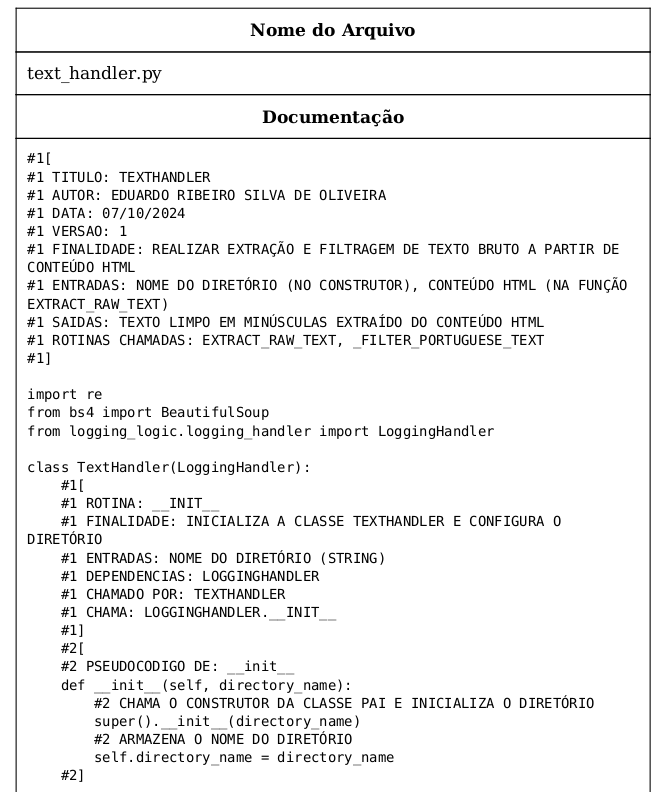
\includegraphics[width=0.7\linewidth]{nivel3.png}
    \caption{Exemplo de visualização de nível 3}
  \end{figure}
\end{frame}

\end{document}